\section{Mise à jour du produit Catia}
\label{majcatia}

\subsection{Principe de fonctionnement}

\par La Fig. \ref{fig:idea} présente la structure type des fichiers de travail : l'idée est de laisser l'utilisateur définir un filaire \textit{ad hoc} dans le produit \texttt{WireframeDefinition.CATProduct} en créant des pièces (\texttt{Wireframe1.CATPart}, \texttt{Wireframe2.CATPart}, ...) avec des projections des points de \texttt{LotusPoints.CATPart}. La macro fait tout simplement une mise à jour des points dans  \texttt{LotusPoints.CATPart} avec les valeurs lus depuis un fichier \texttt{Lotus.dat} et appelle une mise à jour complète du produit \texttt{WireframeDefinition.CATProduct}. 
\par Etant donné que les points du train avant et arrière ont les mêmes noms, \texttt{LotusPoints.CATPART} contiendra deux corps, permettant ainsi de différencier le train avant et arrière lors de la mise à jour.
\par Ensuite, les pièces filaires (\texttt{Wireframe1.CATPart}, \texttt{Wireframe2.CATPart}, ...) peuvent être mises dans un produit séparé (\texttt{Suspension.CATProduct}) pour la conception détaillée. \\

\paragraph{Voici les différents avantages de cette approche:}

\begin{itemize}
    \item définition du filaire \textit{ad hoc} sur un produit dédié : possibilité de définir des nouvelles pièces dans le filaire sans modifier la macro, permettant d'anticiper l'apparition de nouveaux sous-systèmes dans la suspension du véhicule, non présents lors des itérations précédentes (par exemple, ajout d'une barre anti-roulis)
    \item une mise à jour de \texttt{Suspension.CATProduct} ne modifie pas les pièces filaires puisque ces dernières ont été définies dans le contexte de \texttt{WireframeDefinition.CATProduct}: autrement dit la mise à jour des points est indépendante du fichier de conception détaillé
    \item Possibilité d'adapter la construction des pièces filaires aux exigences de forme : placement des repères au centre des pièces
\end{itemize}{}

\begin{figure}
    \centering
    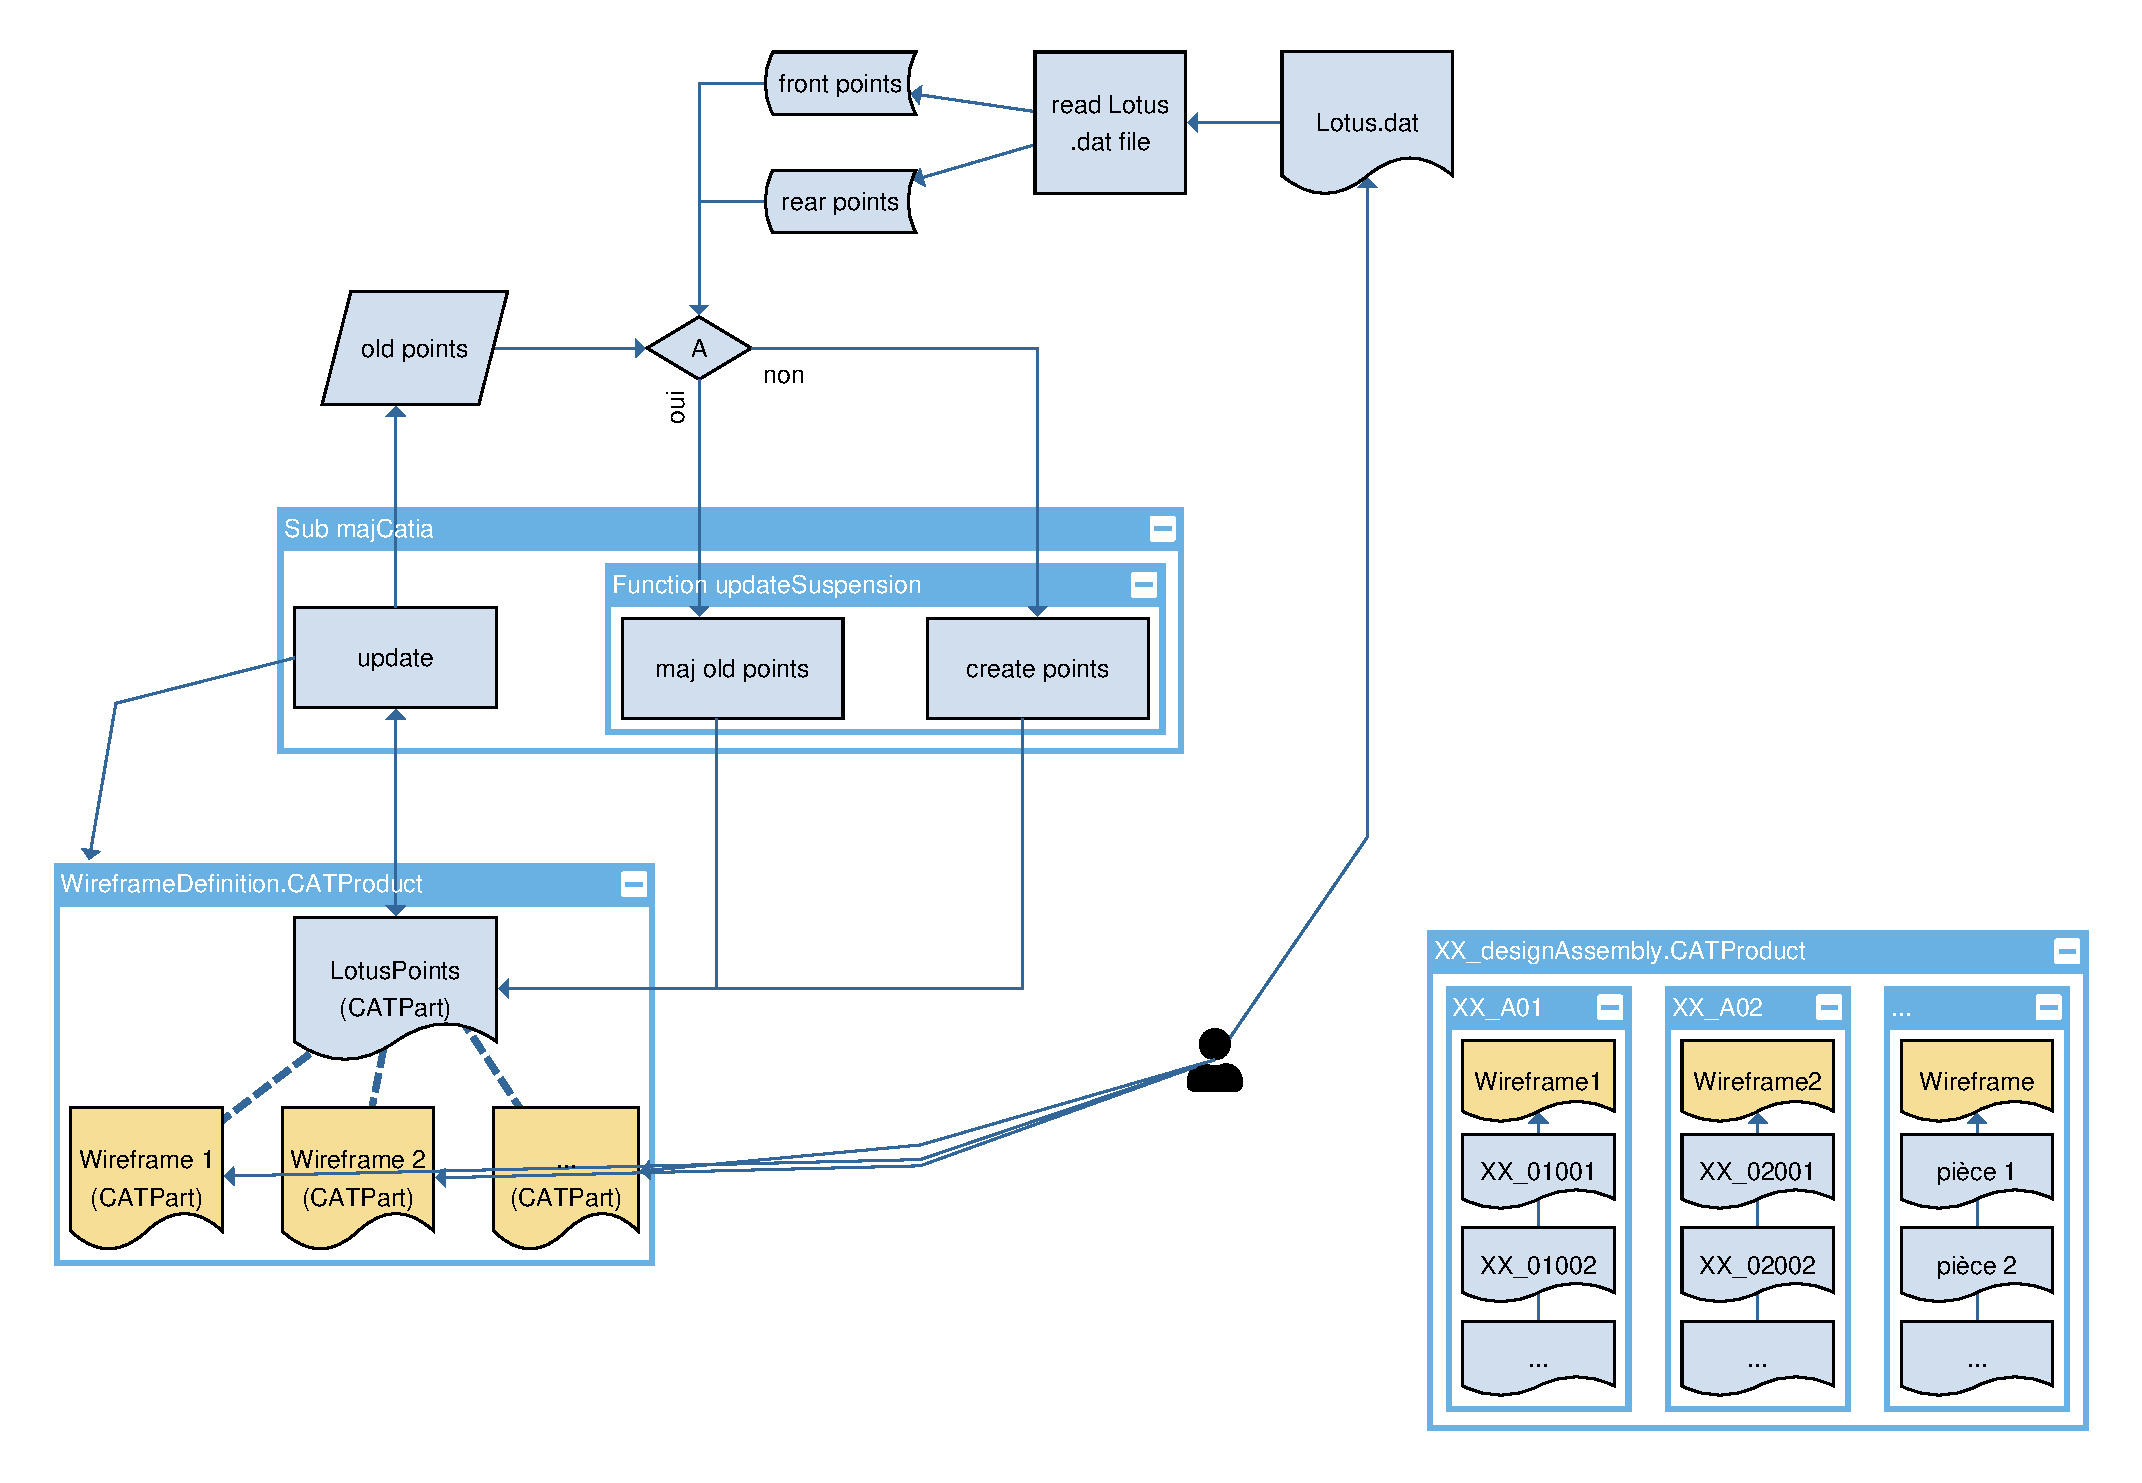
\includegraphics[width=\linewidth]{img/schemaAll.pdf}
    \caption{Représentation schématique du principe de fonctionnement de la macro}
    \label{fig:idea}
\end{figure}

\subsection{Description et organisation du code} %-----------------------------------

\par Dans le module \textit{majCatia}, la subroutine \textit{maj\_Catia} permet de mettre à jour les points présents dans  \texttt{LotusPoints.CATPart} avec les noms et les coordonnées lues depuis le fichier Lotus, comme expliqué dans la section précédente. 

\par Grâce à l'ouverture du produit \texttt{WireframeDefinition.CATProduct}, nous pouvons accéder directement au fichier \texttt{LotusPoints.CATPart}, étant déjà chargé dans la mémoire.
Ainsi, le code fait tout d'abord une scan des points déjà présents dans \texttt{LotusPoints.CATPart} afin de pouvoir distinguer la création d'un nouveau point de la mise à jour d'un point existant. Ensuite, nous faisons une comparaison entre les noms présents dans la liste globale \texttt{frontNames} (créée avec la lecture du ficher Lotus.dat pour le train avant) et \texttt{rearNames} (de manière analogue pour le train arrière) avec ce qui était présent dans les deux corps de \texttt{LotusPoints.CATPart}:
\begin{itemize}
    \item si le point existe déjà, ses coordonnées sont mises à jour en passant par les paramètres de l'objet
    \item sinon, un nouveau point est créé en utilisant la méthode \textit{hybridShapeFactory} et ajouté dans l'arbre de la pièce
\end{itemize}



\par Petit détail concernant la conception à l'EPSA : la conception détaillée est faite par convention sur la partie gauche du véhicule, puis mis en symétrie.
\par Néanmoins, les points Lotus sont définis à droite : nous avons simplement changer le signe de la coordonnée \texttt{Y} afin de réaliser la symétrie.

\subsection{Précautions et points faibles} % ------------------------------------------------------

\par Premièrement, nous remarquons que l'identification des points se base sur leur nom. Pour changer cette propriété, il faut rentrer directement dans le paramétrage du logiciel Lotus. \par On remarque deuxièmement que cette macro ne peut pas effacer des points dans \texttt{LotusPoints.CATPart}.
Pour ce faire, il faut ouvrir manuellement la pièce dans Catia et supprimer les point dans l'arbre. L'intérêt de ceci est d'éviter que la macro efface les mauvais points si l'utilisateur n'est pas précautionneux et nomme de la même manière les nouveaux  points et ceux qu'il a supprimé dans Lotus.
